\documentclass[12pt]{article}
\usepackage[utf8]{inputenc}
\usepackage{polski}
\usepackage{amssymb}
\usepackage{alltt}
\usepackage{float}
\usepackage[a4paper, total={6in, 10in}]{geometry}
\usepackage{listings}
\usepackage{xcolor}
\usepackage{systeme}
\usepackage[usestackEOL]{stackengine}
\usepackage{natbib}
\usepackage{graphicx}
\usepackage{amsmath}
\usepackage{listings}
\usepackage{color} %red, green, blue, yellow, cyan, magenta, black, white
\definecolor{mygreen}{RGB}{28,172,0} % color values Red, Green, Blue
\definecolor{mylilas}{RGB}{170,55,241}
\newcommand{\norm}[1]{\left\lVert#1\right\rVert}
\usepackage{subfigure}
\usepackage{subfig}
\usepackage{minted}


\begin{document}


\lstset{language=Matlab,%
    %basicstyle=\color{red},
    breaklines=true,%
    morekeywords={matlab2tikz},
    keywordstyle=\color{blue},%
    morekeywords=[2]{1}, keywordstyle=[2]{\color{black}},
    identifierstyle=\color{black},%
    stringstyle=\color{mylilas},
    commentstyle=\color{mygreen},%
    showstringspaces=false,%without this there will be a symbol in the places where there is a space
    numbers=left,%
    numberstyle={\tiny \color{black}},% size of the numbers
    numbersep=9pt, % this defines how far the numbers are from the text
    emph=[1]{for,end,break,function},emphstyle=[1]\color{red}, %some words to emphasise
    %emph=[2]{word1,word2}, emphstyle=[2]{style},   
    basicstyle=\ttfamily,
    breaklines=true,
    framextopmargin=50pt,
    frame=single
}

\thispagestyle{empty}
\begin{flushright}{\large Rzeszów, 06.01.2022}
\end{flushright}
\vspace{1.5cm}
\vspace{4.5cm}
\begin{center}
{\large
PODSTAWY MODELOWANIA MATEMATYCZNEGO W INŻYNIERII\par\vspace{2cm}\par
PRACA LABORATORYJNA NR 3\par\vspace{0.2cm}\par
"Nieliniowe modele dynamiczne w postaci układów równań
różniczkowych zwyczajnych i metody ich analizy i rozwiązania."\par\vspace{0.2cm}\par
}

\end{center}
\vspace{8cm}

{\raggedleft\vfill\Longstack[l]{%
  \large Piotr Krawiec L1\vspace{0.2cm} \\
  \large Semestr: 2021/2022 \vspace{0.2cm} \\
  \large Kierunek: III/FS0-DI \vspace{0.2cm} \\
  \large Numer indeksu: 164165 \vspace{0.2cm} \\
  \large Prowadzący: Bohdan Datsko
}\par
}
\vfill


\leavevmode\thispagestyle{empty}\newpage

\tableofcontents

\newpage

\section{Zadania i teoria}
Wykonać modelowanie różnych możliwych typów dynamiki układów \ref{equation-1} i \ref{equation-2}. Otrzymać różne typy rozwiązań układów równań różniczkowych tych równań dla parametrów podanych w tabeli \ref{table-1} zgodnie z zestawem (13).
\begin{table}[H]
\centering
\begin{tabular}{|l|l|l|l|l|l|l|l|l|}
\hline
Numer & A   & $\tau_1$ & $\tau_2$ & b & {\ul A} & $p_1$ & $p_2$ & $p_3$ \\ \hline
13    & 0.5 & 0.2    & 10     & 1 & 4       & 12  & 5   & 13  \\ \hline
\end{tabular}
\caption{Parametry badanych równań}
\label{table-1}
\end{table}

\subsection{Model Bonhoeffer-van der Pol z sześcienną nieliniowością.}
Model ten w standardowej postaci bezwymiarowej wygląda następująco:
\begin{equation}
\begin{split}
\tau \frac{du_1}{dt} = -\frac{1}{3}u_1^{3} + u_1 - u_2  \\
\frac{du_2}{dt} = b u_1 - u_2 + A
\end{split}
\label{equation-1}
\end{equation}
Dla parametru $b=1$ układ ten ma tylko jeden stan stacjonarny:
\begin{equation}
\begin{split}
u_1 = \sqrt[3]{-3A} \\
u_2 = \sqrt[3]{-3A} + A
\end{split}
\label{equation-1}
\end{equation}
Co można wyprowadzić, wychodząc z: 
$$ \frac{du_1}{dt} = 0, \frac{du_2}{dt} = 0 $$
Wyprowadzenie tego wzoru znajduje się poniżej:
\begin{figure}[H]
\centering
    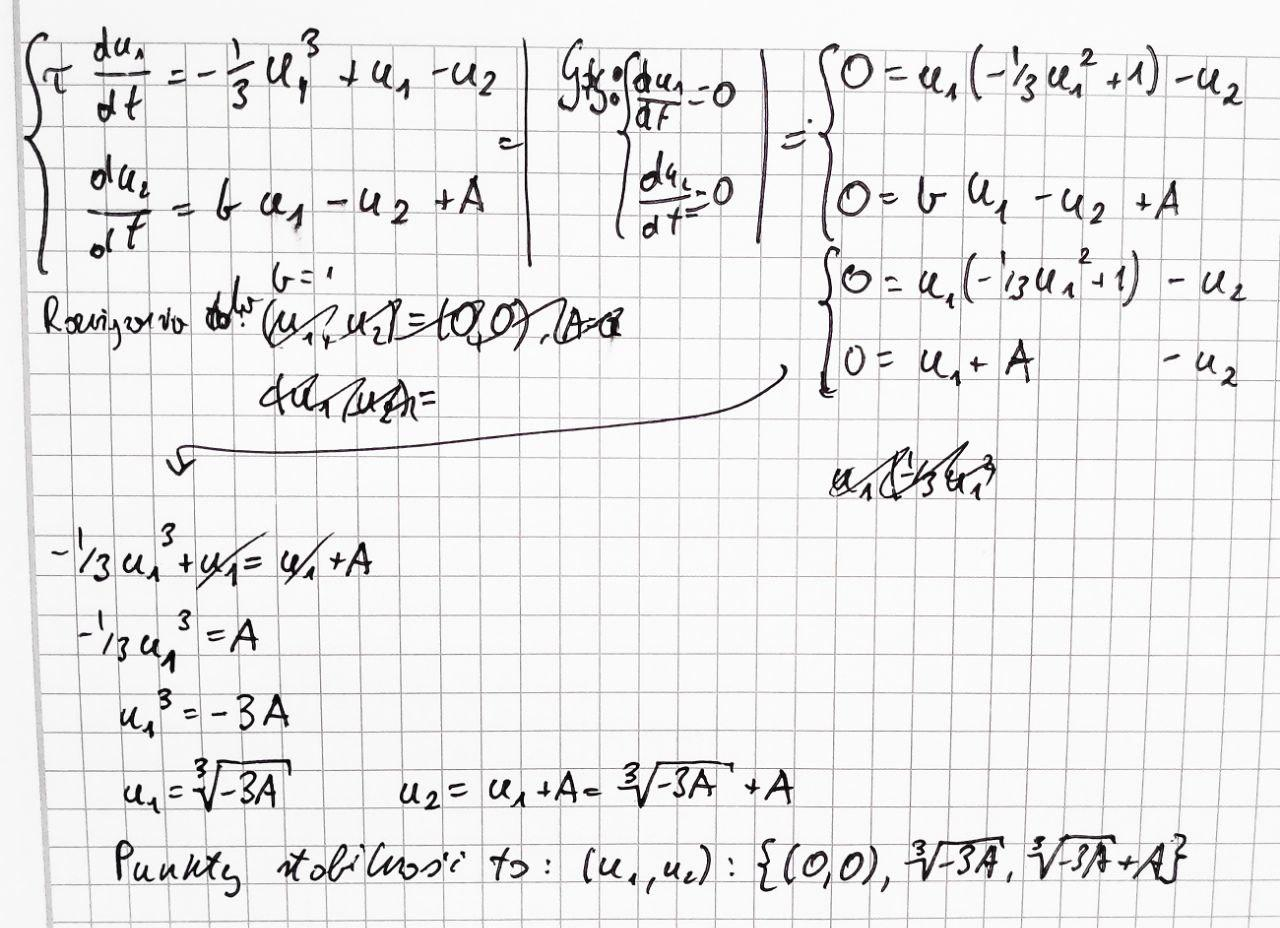
\includegraphics[scale=0.28]{./img/stability-1}
\end{figure}

\subsection{Model Lorentza. Chaotyczna dynamika w nieliniowych układach.}

\begin{equation}
\begin{split}
\frac{du_1}{dt} = \sigma (u_2 - u_1) \\
\frac{du_2}{dt} = u_1 (r - u_3) - u_2 \\
\frac{du_3}{dt} = u_1 u_2 - \beta u_3
\end{split}
\label{equation-2}
\end{equation}




\section{Rozwiązanie w scilab}

\subsection{Model Bonhoeffer-van der Pol z sześcienną nieliniowością w Scilab}

\begin{figure}[H]
\textbf{Rozwiązanie układu dla danych podanych w tabeli}
  \centering
  \begin{minipage}[b]{0.49\textwidth}
    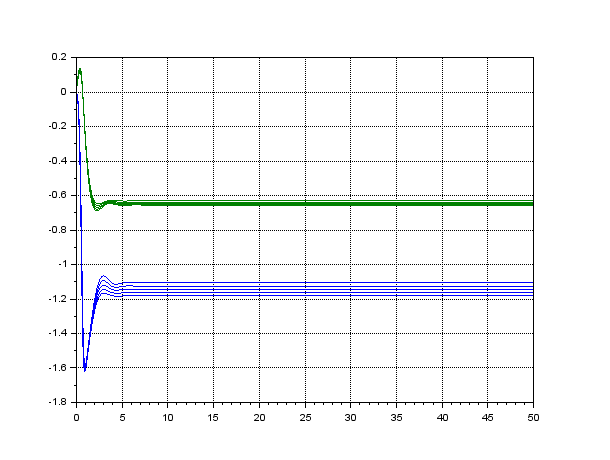
\includegraphics[scale=0.4]{./img/3-1-xy}
    \caption{Wykres u1 i u2 w czasie}
    \end{minipage}
  \hfill
  \begin{minipage}[b]{0.49\textwidth}
    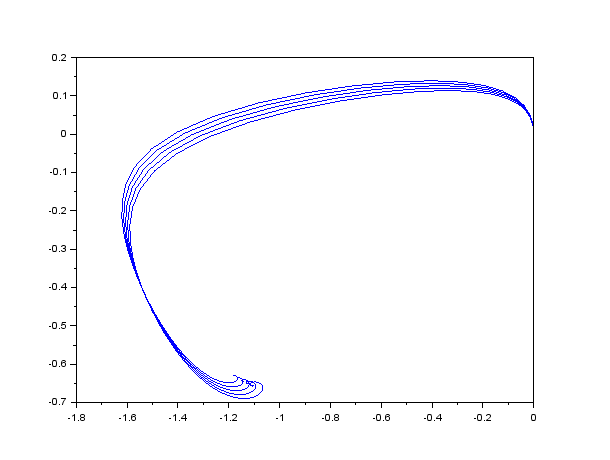
\includegraphics[scale=0.4]{./img/3-1-phase}
    \caption{Wykres fazowy}
    \label{4-analityczne}
  \end{minipage}
\end{figure}

Z powyższych wykresów odczytać możemy, że układ ustabilizował się. Z rozważań teoretycznych możemy obliczyć, że stan stacjonarny to: $$(u_1, u_2) = (\sqrt[3]{-3A}, \sqrt[3]{-3A}+A)$$ i dla danych z tabeli jest to
$$(0.5908329 + 1.0233526i, 1.1408329 + 1.0233526i)$$. Natomiast z wykresu możemy odczytać punkt: 
$$(-1.1816658, -0.6316658)$$. Sprawdzę teraz, jak te wyniki wyglądają w scilab:

\begin{lstlisting}[label={code1},language=scilab,caption={Sprawdzenie wyniku}]
// Teoretyczny punkt stabilny
z = [(-3*A)^(1/3); (-3*A)^(1/3)+A];
 syst2(t, z)
 ans  =

   1.110D-15 + 0.i
   0.        + 0.i

// Punkt w ktorym uklad utknal
 ans  =

  -1.1816658
  -0.6316658
syst2(t, y(:, 1001))
 ans  =
  -1.723D-10
  -0.05   
\end{lstlisting}
Oba te wyniki są zbliżone do 0, czyli różnica ta może wynikać ze sposobu rozwiązania układu. Metoda numeryczna prawdopodobnie znalazła inny punkt stabilny.

\begin{lstlisting}[label={code1},language=scilab,caption={Kod generujący powyższe wykresy}]
tau_1 = 0.2;
b = 1;
A_ = 4;
p_1 = 12;
p_2 = 5;
p_3 = 13;
tau = tau_1;
A = 0.5;

for A = (A-0.1*abs(A)):0.05*abs(A):(A+0.1*abs(A))
    function du=syst2(t, u) //definicja ukladu RR
        du=zeros(2,1);
        du(1)=(-1/3*u(1)^3+u(1)-u(2))/tau;
        du(2)=b*u(1)-u(2)+A;
    endfunction
    x0=[0;0]; t0=0; t=0:0.05:50;y=ode("stiff",x0,t0,t,syst2);
    scf(1);
    plot(t,y); xgrid();
    scf(2);
    plot(y(1,:), y(2,:));
end
xs2png(1, "img/3-1-xy.png")
xs2png(2, "img/3-1-phase.png")
close();close();

u1 = (-3*A)^(1/3)
u2 = u1 + A
\end{lstlisting}

\subsubsection{Modyfikacja parametru $\tau$}
Dla $\tau = 10$ wykresy te wyglądają następująco:

\begin{figure}[H]
\textbf{Rozwiązanie układu dla danych podanych w tabeli i $\tau = 10$}
  \centering
  \begin{minipage}[b]{0.49\textwidth}
    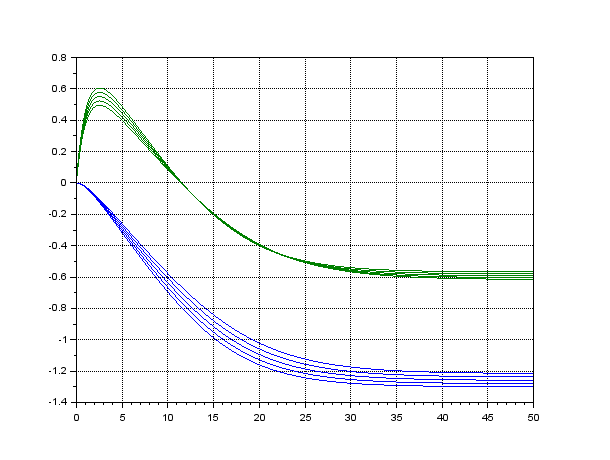
\includegraphics[scale=0.4]{./img/3-1-tau2-xy}
    \caption{Wykres u1 i u2 w czasie}
    \end{minipage}
  \hfill
  \begin{minipage}[b]{0.49\textwidth}
    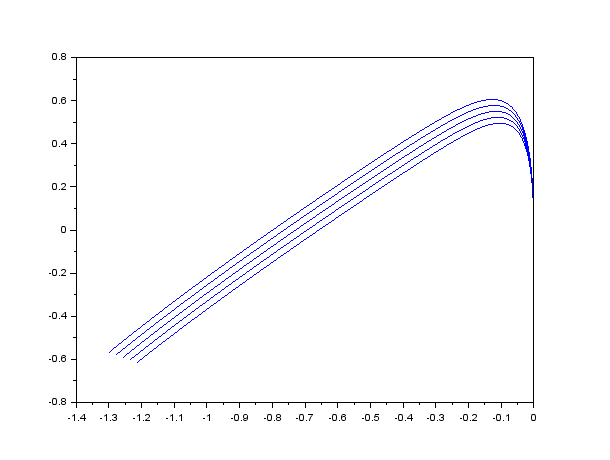
\includegraphics[scale=0.4]{./img/3-1-tau2-phase}
    \caption{Wykres fazowy}
  \end{minipage}
\end{figure}
Tutaj rozwiązanie jest podobnie, jak dla danych z tabeli, w miarę 


\subsubsection{Inne rozwiązania układu}
Poniższe rozwiązania znalazłem zmieniając parametr $A$ w dużym zakresie i sprawdzając, jak zachowuje się układ. Aż natrafiłem na $A=-0.1$. Zmieniając parametr A w zakresie 10 procent, otrzymałem takie wykresy:

\begin{figure}[H]
\textbf{Rozwiązanie układu dla danych podanych w tabeli i $A=-0.1$}
  \centering
  \begin{minipage}[b]{0.49\textwidth}
    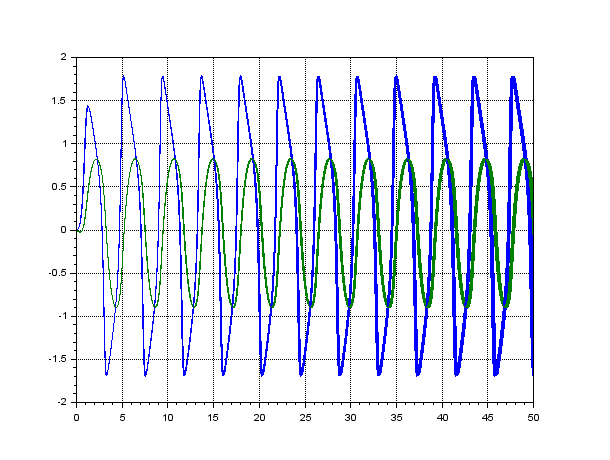
\includegraphics[scale=0.4]{./img/3-1-oscylacje-xy}
    \caption{Wykres u1 i u2 w czasie}
    \end{minipage}
  \hfill
  \begin{minipage}[b]{0.49\textwidth}
    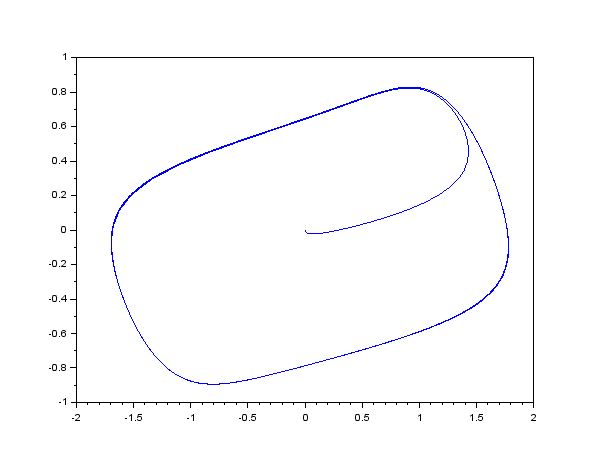
\includegraphics[scale=0.4]{./img/3-1-oscylacje-phase}
    \caption{Wykres fazowy}
  \end{minipage}
\end{figure}

Układ ten wszedł w oscylację. "Szybko" uciekł on z punktu początkowego $(0, 0)$ i zaczął oscylować między punktami stabilności.

\subsection{Model Lorentza. Chaotyczna dynamika w nieliniowych układach.}
\subsubsection{Kod w Scilab}

\begin{lstlisting}[label={code5},language=scilab,caption={Kod generujący powyższe wykresy}]
/////////////////////////////////////// Zadanie 6 //////////
sigma = 10;
b = 8/3;
r = 28;

function du=syst2(t, u)
    du=zeros(3,1);
    du(1)=sigma * (u(2)- u(1))
    du(2)=u(1)*(r - u(3)) - u(2); 
    du(3)=u(1)*u(2) - b *u(3);
endfunction
x0=[1;1;1]; t0=0; t=0:0.05:50;y=ode("stiff",x0,t0,t,syst2);
scf(1);
plot(t,y); xgrid();
scf(2);
plot(y(1,:), y(2,:));
scf(3);
plot(y(1,:), y(3,:));
scf(4);
plot(y(2,:), y(3,:));

xs2png(1, "img/6-111-xy.png")
xs2png(2, "img/6-111-phase-1-2.png")
xs2png(3, "img/6-111-phase-1-3.png")
xs2png(4, "img/6-111-phase-2-3.png")
close(); close(); close(); close();

x0=[-1;-1;-1]; t0=0; t=0:0.05:50;y=ode("stiff",x0,t0,t,syst2);
scf(1);
plot(t,y); xgrid();
scf(2);
plot(y(1,:), y(2,:));
scf(3);
plot(y(1,:), y(3,:));
scf(4);
plot(y(2,:), y(3,:));

xs2png(1, "img/6--111-xy.png")
xs2png(2, "img/6--111-phase-1-2.png")
xs2png(3, "img/6--111-phase-1-3.png")
xs2png(4, "img/6--111-phase-2-3.png")
close(); close(); close(); close();

//////////////////////////////////// Zadanie 7 //////////////////
sigma = 12;
b = 5;
r = 13;

x0=[1;1;1]; t0=0; t=0:0.05:10;y=ode("stiff",x0,t0,t,syst2);
scf(1);
plot(t,y); xgrid();
scf(2);
plot(y(1,:), y(2,:));
scf(3);
plot(y(1,:), y(3,:));
scf(4);
plot(y(2,:), y(3,:));

xs2png(1, "img/7-111-xy.png")
xs2png(2, "img/7-111-phase-1-2.png")
xs2png(3, "img/7-111-phase-1-3.png")
xs2png(4, "img/7-111-phase-2-3.png")
close(); close(); close(); close();

x0=[-20;-20;-20]; t0=0; t=0:0.05:10;y=ode("stiff",x0,t0,t,syst2);
scf(1);
plot(t,y); xgrid();
scf(2);
plot(y(1,:), y(2,:));
scf(3);
plot(y(1,:), y(3,:));
scf(4);
plot(y(2,:), y(3,:));

xs2png(1, "img/7--2011-xy.png")
xs2png(2, "img/7--2011-phase-1-2.png")
xs2png(3, "img/7--2011-phase-1-3.png")
xs2png(4, "img/--2011-phase-2-3.png")
close(); close(); close(); close();
\end{lstlisting}

\subsubsection{Zadanie 6}

Dla obu przedstawionych tutaj punktów początkowych układ ten nie wygasa, co widać na wykresach u1, u2 i u3 w czasie. Widać to także na wykresach fazowych, ponieważ nie ma punktu, w którym układ by się zatrzymał. Powstają charakterystyczne puste miejsca, w które układ nigdy nie wpada.
\vspace{0.5cm}
\begin{center}
\textbf{Rozwiązanie układu dla danych podanych w tabeli i warunków początkowych $u_1'(0)=1$, $u_2'(0)=1$, $u_3'(0)=1$}
\end{center}

\begin{figure}[H]
  \centering
  \begin{minipage}[b]{0.49\textwidth}
    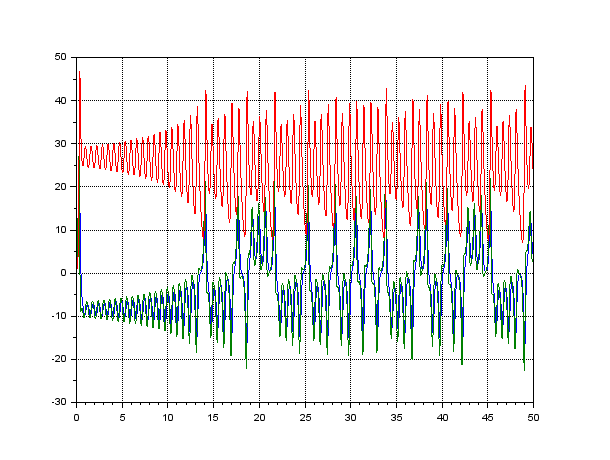
\includegraphics[scale=0.4]{./img/6-111-xy}
    \caption{Wykres u1, u2 i u3 w czasie}
    \end{minipage}
  \hfill
  \begin{minipage}[b]{0.49\textwidth}
    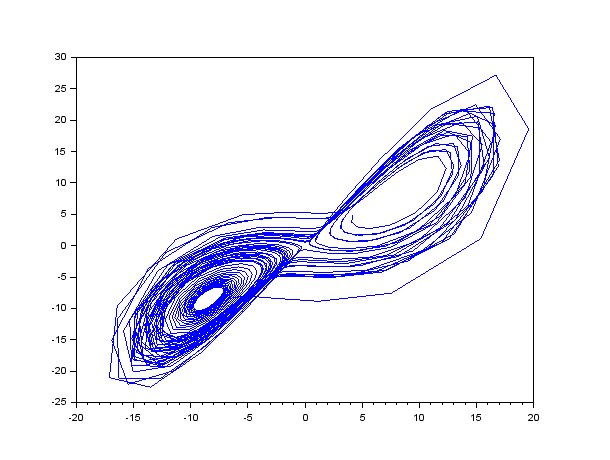
\includegraphics[scale=0.4]{./img/6-111-phase-1-2}
    \caption{Wykres fazowy u1 i u2}
  \end{minipage}
\begin{minipage}[b]{0.49\textwidth}
    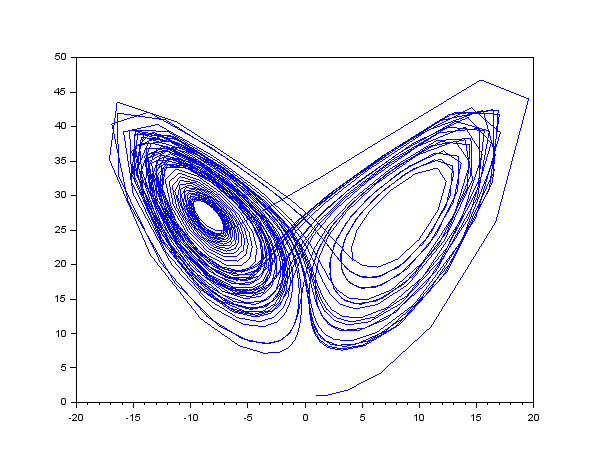
\includegraphics[scale=0.4]{./img/6-111-phase-1-3}
    \caption{Wykres fazowy u1 i u3}
    \end{minipage}
  \hfill
  \begin{minipage}[b]{0.49\textwidth}
    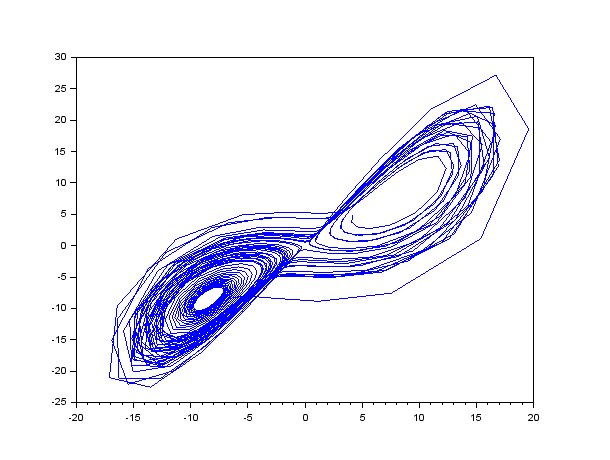
\includegraphics[scale=0.4]{./img/6-111-phase-2-3}
    \caption{Wykres fazowy u2 i u3}
  \end{minipage}
\end{figure}
\newpage
\begin{centering}
\textbf{Rozwiązanie układu dla danych podanych w tabeli i warunków początkowych $u_1'(0)=-1$, $u_2'(0)=-1$, $u_3'(0)=-1$}
\end{centering}
\begin{figure}[H]
  \centering
  \begin{minipage}[b]{0.49\textwidth}
    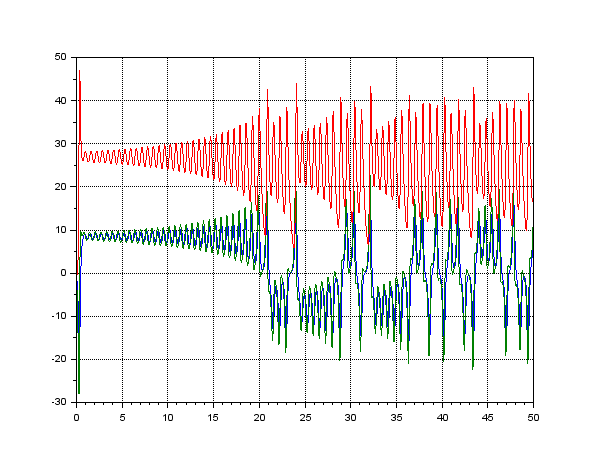
\includegraphics[scale=0.4]{./img/6--111-xy}
    \caption{Wykres u1, u2 i u3 w czasie}
    \end{minipage}
  \hfill
  \begin{minipage}[b]{0.49\textwidth}
    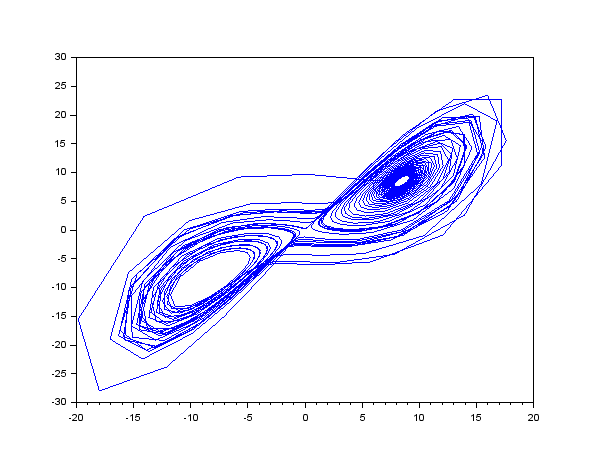
\includegraphics[scale=0.4]{./img/6--111-phase-1-2}
    \caption{Wykres fazowy u1 i u2}
  \end{minipage}
\begin{minipage}[b]{0.49\textwidth}
    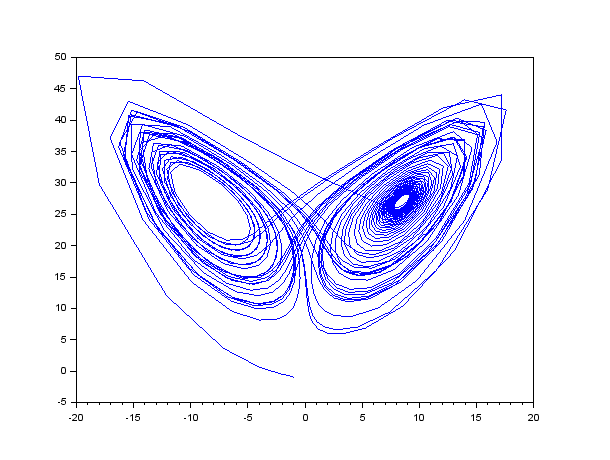
\includegraphics[scale=0.4]{./img/6--111-phase-1-3}
    \caption{Wykres fazowy u1 i u3}
    \end{minipage}
  \hfill
  \begin{minipage}[b]{0.49\textwidth}
    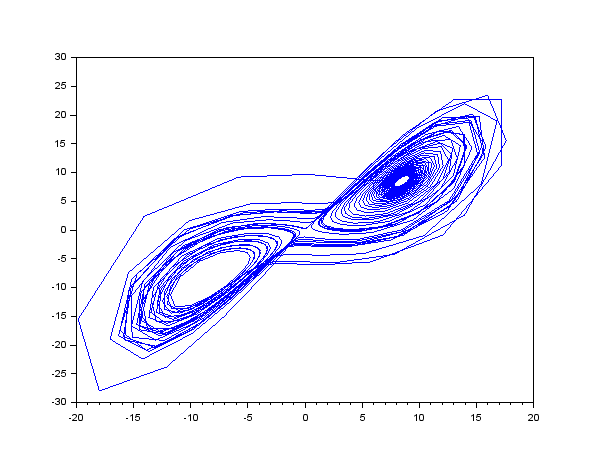
\includegraphics[scale=0.4]{./img/6--111-phase-2-3}
    \caption{Wykres fazowy u2 i u3}
  \end{minipage}
\end{figure}
Zmiana znaków wszystkich parametrów początkowych sprawiła, że wykres stał się swoim lustrzanym obiciem. Punkty wokół, których krąży układ (gęsty i mniej gęsty) zamieniły się miejscami, co nie jest oczywiste, patrząc wyłącznie na pierwszy wykres.

\newpage
\subsubsection{Zadanie 7}
\begin{center}
\textbf{Rozwiązanie układu dla danych $\sigma = 12$, $\beta=5$, $r=13$ i warunków początkowych $u_1'(0)=1$, $u_2'(0)=1$, $u_3'(0)=1$}
\begin{figure}[H]
  \centering
  \begin{minipage}[b]{0.49\textwidth}
    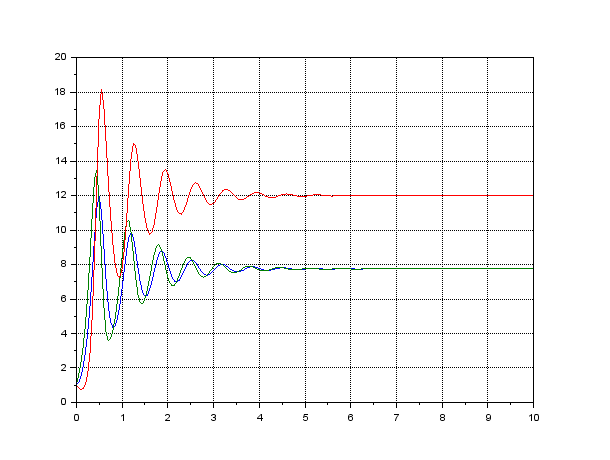
\includegraphics[scale=0.4]{./img/7-111-xy}
    \caption{Wykres u1, u2 i u3 w czasie}
    \end{minipage}
  \hfill
  \begin{minipage}[b]{0.49\textwidth}
    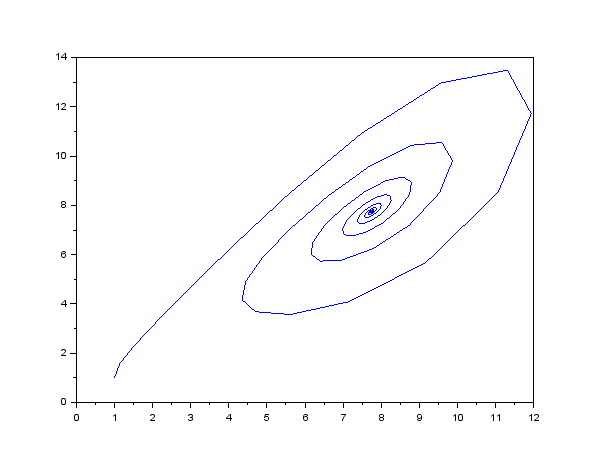
\includegraphics[scale=0.4]{./img/7-111-phase-1-2}
    \caption{Wykres fazowy u1 i u2}
  \end{minipage}
\begin{minipage}[b]{0.49\textwidth}
    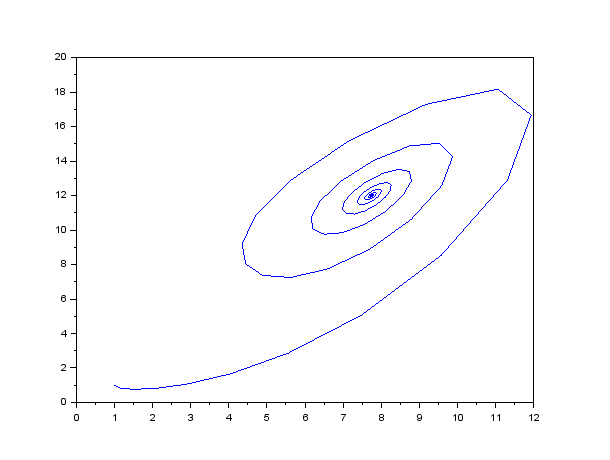
\includegraphics[scale=0.4]{./img/7-111-phase-1-3}
    \caption{Wykres fazowy u1 i u3}
    \end{minipage}
  \hfill
  \begin{minipage}[b]{0.49\textwidth}
    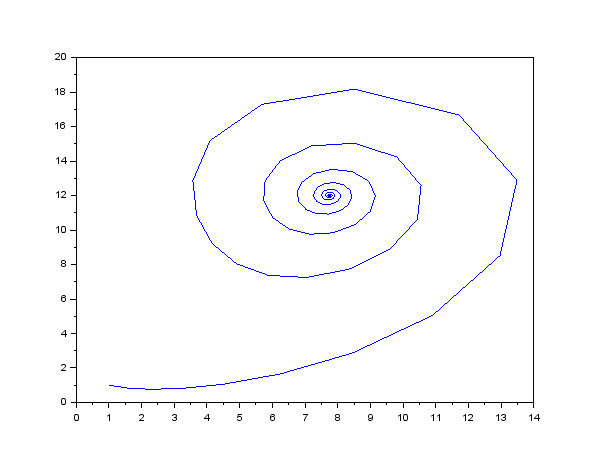
\includegraphics[scale=0.4]{./img/7-111-phase-2-3}
    \caption{Wykres fazowy u2 i u3}
  \end{minipage}
\end{figure}
\end{center}

Po zmianie parametrów układu zmieniła się jego charakterystyka, zamiast oscylować, układ się stabilizuje. Szybkość tej stabilizacji sprawdziłem na następnym rysunku.
\begin{center}
    \textbf{Rozwiązanie układu dla danych $\sigma = 12$, $\beta=5$, $r=13$ i warunków początkowych $u_1'(0)=-20$, $u_2'(0)=-20$, $u_3'(0)=-20$}
\end{center}
\begin{figure}[H]
  \centering
  \begin{minipage}[b]{0.49\textwidth}
    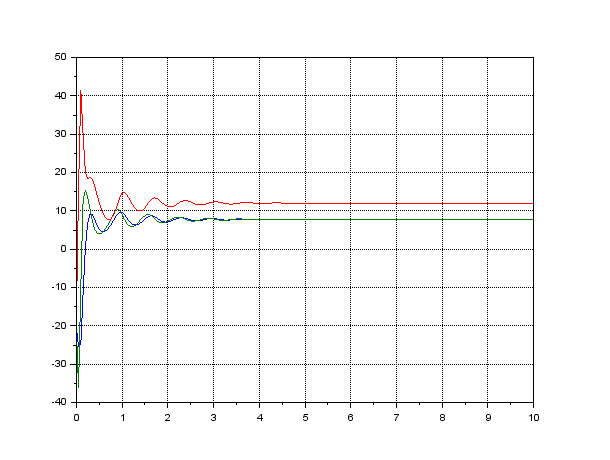
\includegraphics[scale=0.4]{./img/7--2011-xy}
    \caption{Wykres u1, u2 i u3 w czasie}
    \end{minipage}
  \hfill
  \begin{minipage}[b]{0.49\textwidth}
    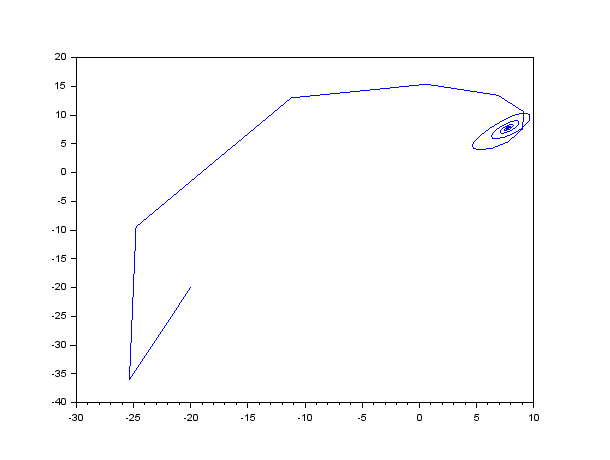
\includegraphics[scale=0.4]{./img/7--2011-phase-1-2}
    \caption{Wykres fazowy u1 i u2}
  \end{minipage}
\begin{minipage}[b]{0.49\textwidth}
    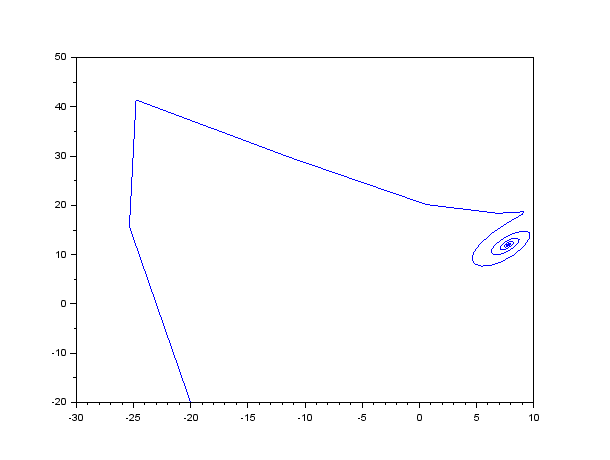
\includegraphics[scale=0.4]{./img/7--2011-phase-1-3}
    \caption{Wykres fazowy u1 i u3}
    \end{minipage}
  \hfill
  \begin{minipage}[b]{0.49\textwidth}
    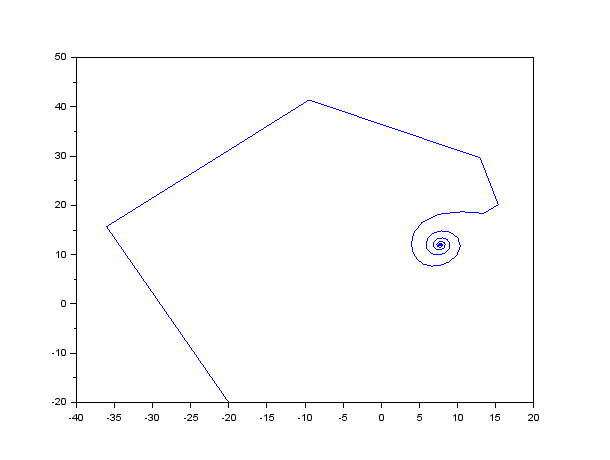
\includegraphics[scale=0.4]{./img/7--2011-phase-2-3}
    \caption{Wykres fazowy u2 i u3}
  \end{minipage}
\end{figure}
Do układu wprowadziłem dosyć duże zaburzenia, tj. ustawiłem duże niezerowe parametry początkowe. Układ ponownie ustabilizował się pomimo dużej zmiany warunków początkowych, ponadto ustabilizował się w podobnym miejscu co układ z parametrami początkowymi $u_1'(0)=1$, $u_2'(0)=1$, $u_3'(0)=1$.

\section{Podsumowanie}
W pracy laboratoryjnej udało się za modelować Model Bonhoeffer-van der Pol z sześcienną nieliniowością jak i Model Lorentza. Dla obu modeli obliczenia numeryczne wykonane w programie Scilab znalazły różne rozwiązania tych układów w zależności od ich parametrów i punktów początkowych. Dla modelu Bonhoeffer-van der Pol z sześcienną nieliniowością znalazłem dwa rozwiązania, tj. układ wygasa lub oscyluje między kilkoma stabilnymi punktami zgodnie z przewidywaniami teoretycznymi omawianymi na wykładzie (patrz rysunki 5 i 6). Podobne zachowania zostały zauważone w drugim układzie, tj. wygasa lub oscyluje. Jednak jego oscylacje przebiegają wokół dwóch punktów. Ponadto bardzo szybko wraca do stabilnego punktu (patrz rysunki 19-22).
\end{document}